\def\utcp{$u$TCP\xspace}
\def\utls{$u$TLS\xspace}
\def\ucobs{$u$COBS\xspace}

As the Internet has grown and evolved
over the past few decades,
congestion control algorithms and extensions such as MPTCP
continue to reflect an evolving TCP.
However,
a proliferation of middleboxes
such as 
Network Address Translators (NATs), 
Firewalls,
and 
Performance Enhancing Proxies (PEPs),
has arguably stretched the waist of the Internet hourglass
upwards from IP
to include
TCP and UDP~\cite{rosenberg08udp, ford08breaking, popa10http},
making it increasingly difficult
to deploy new transports
and to
use anything but TCP and UDP 
on the Internet.

TCP~\cite{rfc793} was originally designed to offer applications
a convenient, high-level communication abstraction
with semantics emulating Unix file I/O or pipes:
a reliable, ordered bytestream,
through an end-to-end channel (or connection).
As the Internet has evolved, however,
applications needed better abstractions
from the transport.
We start this section by examining
how TCP's role in the network has evolved
from a communication {\em abstraction} to a communication {\em substrate},
why its in-order delivery model makes TCP a poor substrate,
why other OS-level transports have failed to replace TCP in this role,
and why UDP is inadequate as the only alternative substrate to TCP.

\subsection{Rise of Application-Level Transports}

The transport layer's traditional role in a network stack
is to build high-level communication abstractions
convenient to applications,
atop the network layer's basic packet delivery service.
TCP's reliable, stream-oriented design~\cite{rfc793}
exemplified this principle,
by offering an inter-host communication abstraction
modeled on Unix pipes,
which were the standard {\em intra-host} communication abstraction
at the time of TCP's design.
The Unix tradition of
implementing TCP in the OS kernel
offered further convenience,
allowing much application code to ignore the difference between
an open disk file, an intra-host pipe, or an inter-host TCP socket.

\begin{figure}[tbp]
\centering
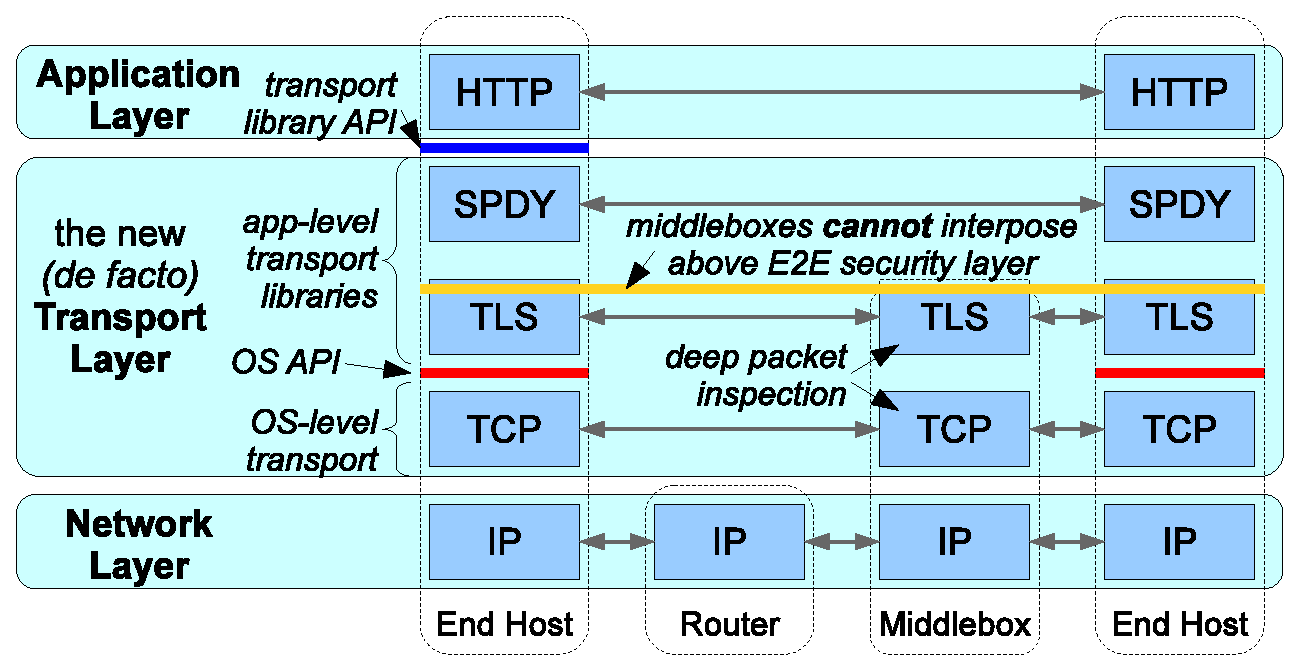
\includegraphics[width=0.8\textwidth]{figures/layers.eps}
\caption{Today's ``{\em de facto} transport layer''
	is effectively split between OS and application code. (taken from
    \cite{nowlan12fitting})}
\label{f:layers}
\end{figure}

Instead of building directly atop
traditional OS-level transports such as TCP or UDP, however,
today's applications
frequently introduce additional transport-like
protocol layers at user-level,
typically implemented via application-linked libraries.
Examples include the ubiquitous SSL/TLS~\cite{rfc5246},
media transports such as RTP~\cite{rfc3550},
and experimental multi-streaming transports such as
SST~\cite{ford07structured}, SPDY~\cite{spdy},
and \O{}MQ~\cite{zeromq}.
Applications increasingly use HTTP or HTTPS over TCP
as a substrate~\cite{popa10http};
this is also illustrated by 
the W3C's WebSocket interface~\cite{websocket},
which offers general bidirectional communication
between browser-based applications and Web servers atop HTTP and HTTPS.

In this increasingly common design pattern,
the ``transport layer'' as a whole has in effect become
a stack of protocols straddling the OS-application boundary.
Figure~\ref{f:layers} illustrates one example stack,
representing Google's experimental Chrome browser,
which inserts SPDY for multi-streaming and TLS for security
at application level,
atop the OS-level TCP.

One can debate whether a given application-level protocol
fits some definition of ``transport'' functionality.
The important point, however,
is that {\em today's applications no longer need, or expect,
the underlying OS to provide ``convenient'' communication abstractions:
an application simply links in libraries, frameworks,
or middleware offering the abstractions it desires.}
What today's applications
need from the OS is not convenience,
but {\em an efficient substrate}
atop which application-level libraries
can build the desired abstractions.

\subsection{TCP's Latency Tax}

While TCP has proven to be a popular
substrate for application-level transports,
using TCP in this role
converts its delivery model from a blessing into a curse.
Application-level transports are just as capable as the kernel
of sequencing and reassembling packets into
a logical data unit or ``frame''~\cite{clark90architectural}.
By delaying any segment's delivery to the application
until all prior segments are received and delivered, however,
TCP imposes a ``latency tax'' on all segments
arriving within one round-trip time (RTT) after any single lost segment.

This latency tax is a fundamental byproduct
of TCP's in-order delivery model,
and is irreducible,
in that an application-level transport
cannot ``claw back''
the time a potentially useful segment
has wasted in TCP's buffers.
The best the application can do is
simply to {\em expect} higher latencies to be common.
A conferencing application can use a longer jitter buffer,
for example,
at the cost of increasing user-perceptible lag.
Network hardware advances are unlikely to address this issue, 
since TCP's latency tax depends on RTT,
which is lower-bounded by the speed of light
for long-distance communications.

\subsection{Alternative OS-level Transports}
\label{sec:motiv-alts}

All standardized OS-level transports since TCP, including
	UDP~\cite{rfc768}, RDP~\cite{rfc908},
	DCCP~\cite{rfc4340}, and SCTP~\cite{rfc4960},
support out-of-order delivery.
The Internet's evolution has created strong barriers
against the widespread deployment of new transports
other than the original TCP and UDP, however.
These barriers are detailed elsewhere~\cite{
	rosenberg08udp,ford08breaking,popa10http},
but we summarize two key issues here.

First, 
adding or enhancing a ``native'' transport built atop IP
involves modifying popular OSes,
effectively increasing the bar for widespread deployment
and making it 
more difficult to evolve transport functionality
below the red line representing the OS API
in Figure~\ref{f:layers}.
Second, the Internet's original ``dumb network'' design,
in which routers that ``see'' only up to the IP layer,
has evolved into a ``smart network''
in which pervasive middleboxes
perform deep packet inspection and interposition
in transport and higher layers.
Firewalls tend to block ``anything unfamiliar'' for security reasons,
and Network Address Translators (NATs)
rewrite the port number in the  transport header,
making both incapable of allowing traffic from a new transport
without explicit support for that transport.
Any packet content
not protected by end-to-end security such as TLS---%
the yellow line in Figure~\ref{f:layers}---%
has become ``fair game''
for middleboxes to inspect and interpose on~\cite{
	reis08detecting},
making it more difficult to evolve transport functionality
anywhere below that line.


\subsection{Why Not UDP?}

As the only widely-supported transport
with out-of-order delivery,
UDP offers a natural
substrate for application-level transports.
Even applications otherwise well-suited to UDP's delivery model
often favor TCP as a substrate, however.

A recent study found over 70\% of streaming media using TCP~\cite{
	guo06delving},
and even latency-sensitive conferencing applications
such as Skype
often use TCP~\cite{baset06analysis}.
Firewalls can monitor the TCP state machine
to help thwart network attacks~\cite{handley01network},
but determining an application session's state atop UDP
requires application-specific analysis~\cite{northcutt05inside},
creating an incentive for firewalls to block UDP in general.

In general,
network middleboxes support UDP widely but not {\em universally}.
For this reason,
latency-sensitive applications
seeking maximal connectivity ``in the wild''
often fall back to TCP when UDP connectivity fails.
Skype~\cite{baset06analysis}
and Microsoft's Direct\-Access VPN~\cite{davies09directaccess},
for example,
support UDP but can masquerade
as HTTP or HTTPS streams atop TCP when required for connectivity.

TCP can offer performance advantages over UDP as well.
For applications requiring congestion control,
an OS-level implementation in TCP
may be more timing-accurate
than an application-level implementation in a UDP-based protocol,
because the OS kernel
can avoid the timing artifacts of 
system calls and process scheduling~\cite{zec02estimating}.
Hardware TCP offload engines
can optimize common-case efficiency
in end hosts~\cite{mogul03tcp},
and performance enhancing proxies
can optimize TCP throughput across diverse networks~\cite{
	rfc3234,cisco-rbscp}.
Since middleboxes can track TCP's state machine,
they impose much longer idle timeouts on open TCP connections---%
nominally two hours~\cite{rfc5382}---%
whereas UDP-based applications must send keepalives
every two minutes to keep an idle connection open~\cite{rfc4787},
draining power on mobile devices.

\subsection{Breaking Out Of the Transport Logjam}
Applications and application developers care most about 
services that the networking infrastructure offers to them
and not how packets look on the wire;
that is, they care about 
new transport {\em services}, not new transport {\em protocols}.
On the other hand,
middleboxes care most about how packets look on the wire,
and generally do not care about what services are offered to the applications;
that is, changing the transport protocol's bits on the wire
will require changing middleboxes to respond to these changes as well.

For application developers,
TCP versus UDP represents an ``all-or-nothing'' choice
on the spectrum of services applications need.
Applications desiring some but not all of TCP's services,
such as congestion control but unordered delivery,
must reimplement and tune all other services atop UDP
or suffer TCP's performance penalties.

Without dismissing UDP's usefulness 
as a truly ``least-common-denominator'' substrate,
we believe the factors above
suggest that TCP will also remain a popular substrate---%
even for latency-sensitive applications
that can benefit from out-of-order delivery---%
and that a deployable, backward-compatible workaround
to TCP's latency tax
can significantly benefit such applications.

Recognizing that the development of application-level transports
and the use of TCP as a substrate under them
is likely to continue and expand,
we now describe {\em Minion},
an architecture for efficient but backward-compatible
unordered delivery over extant transports, including TCP.
Minion consists of
{\em \utcp},
a small OS extension
adding basic unordered delivery primitives to TCP,
and two application-level protocols
implementing datagram-oriented delivery services
that function on either \utcp or unmodified TCP stacks.

While building a new transport on UDP 
or using alternative OS-level transports where available
are both perfectly reasonable design approaches,
Minion offers a uniform interface for applications to use
along with an alternative option
where the ubiquitous TCP protocol is adequate, but the sockets API is not;
where a new transport service
can be offered using TCP's bits on the wire.

\subsection{Minion Architecture Overview}

Minion is an architecture and protocol suite
designed to provide efficient unordered delivery built atop
existing transports.
Minion itself offers no high-level abstractions:
its goal is to serve
applications and higher application-level transports,
by acting as a ``packhorse''
carrying raw datagrams as reliably and efficiently as possible
across today's diverse and change-averse Internet.

\begin{figure}[tbp]
\centering
\includegraphics[width=0.6\textwidth]{figures/minionarch.eps}
\caption{Minion architecture (taken from~\cite{nowlan12fitting})}
\label{f:minionarch}
\end{figure}

Figure~\ref{f:minionarch} illustrates Minion's architecture.
Applications and higher application-level transports
link in and use Minion in the same way as they already use
existing application-level transports
such as DTLS~\cite{rfc4347},
the datagram-oriented analog of SSL/TLS~\cite{rfc5246}.
In contrast with DTLS's goal of layering security
atop datagram transports such as UDP or DCCP,
Minion's goal is to offer efficient datagram delivery
atop {\em any} available OS-level substrate, including TCP.

Minion consists of
several application-level transport protocols,
%in the spirit of Section~\ref{sec:motiv},
together with a set of optional enhancements
to end hosts' OS-level TCP implementations.

Minion's enhanced OS-level TCP stack,
called {\em \utcp} (``unordered TCP''),
includes sender- and receiver-side
API features supporting unordered delivery and prioritization,
as detailed later in this section.
These enhancements affect only the OS API
through which application-level transports such as Minion
interact with the TCP stack,
and make {\em no} changes to TCP's wire protocol.

Minion's application-level protocol suite currently consists
of the following main components:
\begin{itemize}
\item	{\bf \ucobs} is a protocol
	that implements a minimal unordered datagram delivery service
	atop either unmodified TCP or \utcp,
	using 
    {\em Consistent-Overhead Byte Stuffing}, or
    COBS encoding~\cite{cheshire97consistent}
	to facilitate out-of-order datagram delimiting
	and prioritized delivery,
	as described later in Section~\ref{sec:dgrams_utcp}.
\item	{\bf \utls} is a modification of
	the traditionally stream-oriented TLS~\cite{rfc5246},
	offering a secure, unordered datagram delivery service
	atop TCP or \utcp.
	The wire-encoding of \utls streams
	is designed to be indistinguishable in the network
	from conventional, encrypted TLS-over-TCP streams (e.g., HTTPS),
	offering a maximally conservative design point
	that makes no network-visible changes
	``below the yellow line''
	in Figure~\ref{f:minionarch}.
	Section~\ref{sec:dgrams_utcp} describes \utls.
\item	Minion adds shim layers
	atop OS-level datagram transports, such as UDP and DCCP,
	to offer applications a consistent API
	for unordered delivery across multiple OS-level transports.
	Since these shims are merely wrappers
	for OS transports already offering unordered delivery,
	this paper does not discuss them in detail.
\end{itemize}

Minion currently leaves to the application
the decision of {\em which} protocol to use for a given connection:
e.g., \ucobs or \utls atop TCP/\utcp,
or OS-level UDP or DCCP via Minion's shims.
Other ongoing work explores {\em negotiation protocols}
to explore the protocol configuration space dynamically,
optimizing protocol selection and configuration
for the application's needs and the network's 
constraints~\cite{ford09efficient}.
Many applications already incorporate simple negotiation schemes,
however---%
e.g., attempting a UDP connection first
and falling back to TCP if that fails---%
and adapting these mechanisms
to engage Minion's protocols according to
application-defined preferences and decision criteria
should be straightforward.

\subsection{Compatibility and Deployability}

Minion addresses the key barriers to transport evolution,
outlined in Section~\ref{sec:motiv-alts},
by creating a backward-compatible, incrementally deployable substrate
for new application-layer transports desiring unordered delivery.
Minion's deployability rests on the fact that it can,
when necessary,
avoid relying on changes either
``below the red line'' in the end hosts
(the OS API in Figure~\ref{f:minionarch}),
or
``below the yellow line'' in the network
(the end-to-end security layer in Figure~\ref{f:minionarch}).

While Minion's \ucobs and \utls protocols
offer maximum performance benefits from out-of-order delivery
when both endpoints include OS support for Minion's \utcp enhancements,
\ucobs and \utls still function and interoperate correctly
even if neither endpoint supports \utcp,
and the application need not know or care
whether the underlying OS supports \utcp.
If only one endpoint OS supports \utcp,
Minion still offers incremental performance benefits,
since \utcp's sender-side and receiver-side enhancements are independent.
A \ucobs or \utls connection atop a mixed TCP/\linebreak[0]\utcp endpoint-pair
benefits from \utcp's sender-side enhancements
for datagrams sent by the \utcp endpoint,
and the connection benefits from \utcp's receiver-side enhancements
for datagrams arriving at the \utcp host.

Addressing the challenge of network-compatibility
with middleboxes that filter new OS-level transports
and sometimes UDP,
Minion offers application-level transports
a continuum of substrates
representing different tradeoffs
between suitability to the application's needs
and compatibility with the network.

An application can use unordered OS-level transports
such as UDP, DCCP~\cite{rfc4340}, or SCTP~\cite{rfc4960},
for paths on which they operate,
but Minion offers an unordered delivery alternative
wire-compatible not only with TCP,
but with the ubiquitous TLS-over-TCP streams
on which HTTPS (and hence Web security and E-commerce) are based,
likely to operate in almost any network environment
purporting to offer ``Internet access.''

\subsection{Minion's Unordered Delivery using TCP and TLS}
We now briefly discuss Minion's true unordered delivery
over bytestream protocols;
we describe how Minion provides true unordered datagram
delivery without modifying the TCP and TLS wire-formats.

Minion enhances the OS's TCP stack
with API enhancements supporting unordered delivery
in both TCP's send and receive paths,
enabling applications to reduce transmission latency
at both the sender- and receiver-side end hosts
when both endpoints support \utcp.
Since \utcp makes no change to TCP's wire protocol,
two endpoints need not ``agree'' on whether to use \utcp:
one endpoint gains latency benefits from \utcp
even if the other endpoint does not support it.
Further, an OS may choose independently
whether to support the sender- and receiver-side enhancements,
and when available, applications can activate them independently.

\utcp does {\em not} seek to offer
``convenient'' or ``clean'' unordered delivery abstractions
directly at the OS API.
Instead, \utcp's design is motivated by the goals of
maintaining exact compatibility
with TCP's existing wire-visible protocol and behavior,
and facilitating deployability
by minimizing the extent and complexity
of changes to the OS's TCP stack.

\subsubsection{\utcp: Receiver-Side Modifications}

A conventional TCP receiver delivers data in-order 
to the receiving application,
holding back any data that is received out of order.
\utcp modifies the TCP receive path,
enabling a receiving application
to request immediate delivery of data 
that is received by \utcp,
both in order and out of order.

\utcp makes two modifications to a conventional TCP receiver.
First, whereas a conventional TCP stack
delivers received data to the application
only when prior gaps in the TCP sequence space are filled,
the \utcp receiver
makes data segments available to the application immediately upon receipt,
skipping TCP's usual reordering queue.
The data the \utcp stack delivers to the application
in successive application reads
may skip forward and backward in the transmitted byte stream,
and \utcp may even deliver portions
of the transmitted stream multiple times.
\utcp guarantees only that the data returned by each application read
corresponds to {\em some} contiguous sequence of bytes
in the sender's transmitted stream.

Second,
when servicing an application's read,
the \utcp receiver also delivers the logical offset
of the first returned byte
in the sender's original byte stream---information 
that a TCP receiver must maintain to arrange received segments in order.

\begin{figure}[htb]
\centering
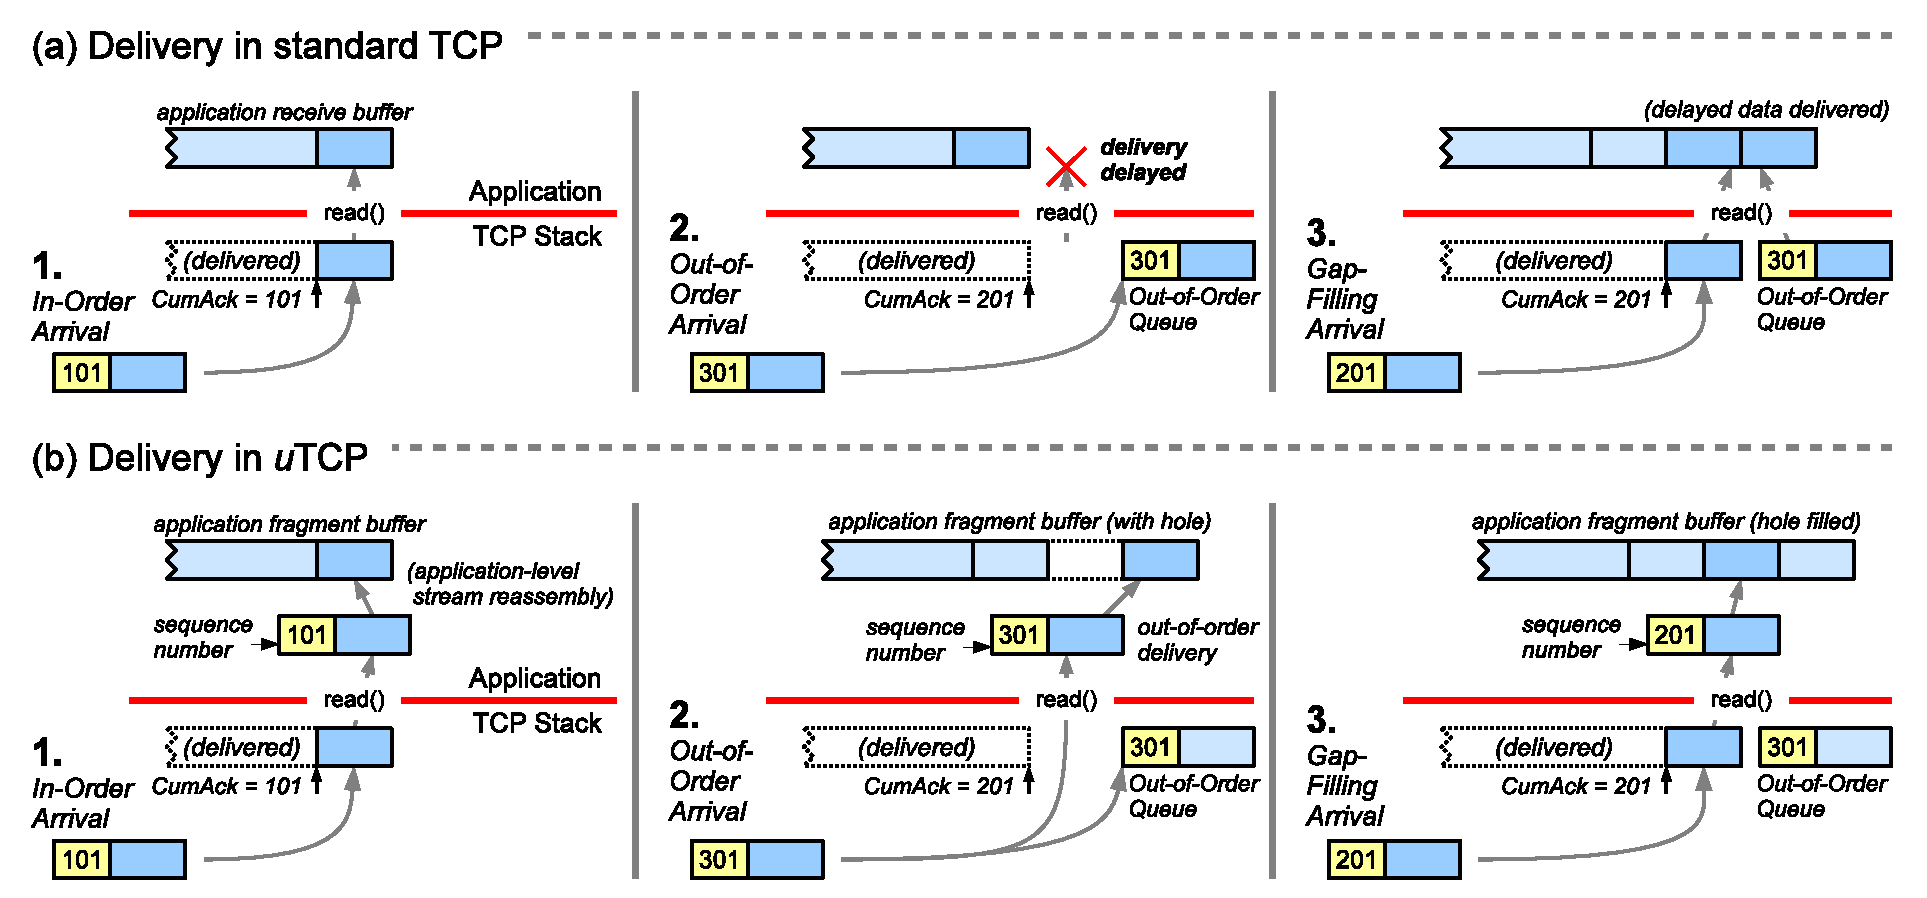
\includegraphics[width=0.99\textwidth]{figures/utcpdelivery.eps}
\caption{
Delivery behavior of (a) standard TCP, and (b) \utcp,
upon receipt of in-order and out-of-order segments.
(taken from~\cite{nowlan12fitting})}
\label{f:utcpdelivery}
\end{figure}

Figure~\ref{f:utcpdelivery} illustrates \utcp's receive-side behavior,
in a simple scenario
where three TCP segments arrive in succession:
first an in-order segment, then an out-of-order segment,
and finally a segment filling the gap between the first two.
With \utcp,
the application receives each segment as soon as it arrives,
along with the sequence number information it needs to reconstruct
a complete internal view of
whichever fragments of the TCP stream have arrived.

\subsubsection{\utcp: Sender-Side Modifications}
While \utcp's receiver-side enhancements
address the ``latency tax''
on segments waiting in TCP's reordering buffer,
TCP's sender-side queue can also introduce latency,
as segments the application has already written to a TCP socket---%
and hence ``committed'' to the network---%
wait until TCP's flow and congestion control
allow their transmission.
Many applications can benefit from the ability to ``late-bind''
their decision on {\em what} to send until the last possible moment,
and also from being able to transmit a message of higher priority
that bypasses any lower priority messages in the sender-side queue.

A \utcp sender allows a sending application
to specify a tag with each application write,
which the \utcp sender currently
interprets as a priority level.
Instead of unconditionally placing the newly-written data
at the tail of the send queue as TCP normally would,
\utcp{} {\em inserts} the newly-written data into the send queue
just {\em before} any lower-priority data
in the send queue not yet transmitted.

With these modifications to a TCP stack,
none of which require changes to the TCP wire-format,
\utcp offers an interface which,
while not convenient for applications, 
is powerful.
In the next Section,
we discuss how we build a userspace library that uses this interface
that provides a simple unordered delivery service,
unordered delivery of encrypted messages,
and logically separate data streams 
within a single \utcp connection.

\subsubsection{Datagrams atop \utcp}
\label{sec:dgrams_utcp}

Applications built on datagram substrates such as UDP
generally assume the underlying layer preserves datagram boundaries.
TCP's stream-oriented semantics do not preserve
any application-relevant frame boundaries within a stream, however.
Both the TCP sender and network middleboxes can and do
coalesce TCP segments or re-segment TCP streams
in unpredictable ways~\cite{honda2011still}.

Atop \utcp,
a userspace library can reconstruct contiguous fragments 
in the received data stream
using the metadata sequence number information 
that \utcp passes along at the receiver.
However,
providing unordered message delivery service atop \utcp
requires delimiting application messages in the bytestream.
While record delimiting is commonly done
by application protocols such as HTTP, SIP, and many others,
a key property that we require to provide a true unordered delivery service
is that a receiver must be able to extract a given message 
independently of other messages.
That is, 
as soon as a complete message is received,
the message delimiting mechanism must
allow for extraction of the message from the bytestream fragment,
without relying on the receipt of earlier messages.

Minion implements self-delimiting messages in two ways:
\begin{enumerate}
    \item To encode application datagrams efficiently, 
    the userspace library employs 
    {\em Consistent-Overhead Byte Stuffing}, or
    COBS~\cite{cheshire97consistent}
    to delimit and extract messages.
    COBS is a binary encoding
    which eliminates {\em exactly} one byte value from a record's encoding
    with minimal bandwidth overhead.
    To encode an application record,
    COBS first scans the record for {\em runs}
    of contiguous marker-free data followed by exactly one marker byte.
    COBS then removes the trailing marker,
    instead {\em prepending} a non-marker byte indicating the run length.
    A special run-length value indicates a run of 254 bytes
    {\em not} followed by a marker in the original data,
    enabling COBS to divide arbitrary-length runs into 254-byte runs
    encoded into 255 bytes each,
    yielding a worst-case expansion of only 0.4\%.

    \item The userspace library 
    coaxes out-of-order delivery from
    the {\em existing} TCP-oriented TLS wire format,
    producing an encrypted datagram substrate
    indistinguishable on the wire from standard TLS connections.
    TLS~\cite{rfc5246} already breaks its communication into {\em records},
    encrypts and authenticates each record,
    and prepends a header
    for transmission on the underlying TCP stream.
    TLS was designed to decrypt records strictly in-order, however,
    creating challenges 
    which the userspace library overcomes~\cite{nowlan12fitting}.
    Run on port 443,
    our encrypted stream atop \utcp is indistinguishable from HTTPS---%
    regardless of whether the application actually uses HTTP headers,
    since the HTTP portion of HTTPS streams are TLS-encrypted anyway.
    Deployed this way,
    Minion effectively offers an end-to-end protected substrate
    in the ``HTTP as the new narrow waist'' philosophy~\cite{popa10http}.
\end{enumerate}

\subsection{Impact on Real Applications}

Minion's unordered delivery service 
benefits a number of applications;
we refer the reader to detailed discussion and experiments 
in~\cite{nowlan12fitting}.
Of these applications,
we briefly discuss how Minion fits within
ongoing efforts to develop a next-generation transport for the web,
such as SPDY\cite{spdy} and the Internet Engineering Task Force (IETF)'s 
HTTP/2.0 (httpbis) effort.
Developing a next-generation HTTP 
requires either submitting to TCP's latency tax
for backward compatibility,
as with SPDY's use of TLS/TCP,
or developing and deploying new transports atop UDP,
neither of which,
as we discussed earlier in this section,
is a satisfying alternative.

Minion bridges this gap 
and demonstrates that it is possible to obtain
unordered delivery from wire-compatible TCP and TLS streams
with surprisingly small changes to TCP stacks
and application-level code.
These protocols offer latency-sensitive applications
performance benefits comparable to UDP or DCCP,
with the compatibility benefits of TCP and TLS.
Without discounting the value of UDP and newer OS-level transports,
Minion offers a more conservative path toward
the performance benefits of unordered delivery,
which we expect to be useful to applications
that use TCP for a variety of pragmatic reasons.

%\subsection{Editorial Note}
%Some of the text and figures in this Section have been adapted from
%the following two publications: